\documentclass[../main/main.tex]{subfiles}
\begin{document}
\chapter{Result benchmark}
	
In this chapter we present the benchmark between the integrator already available in \texttt{VegasFlow} and different variations of the VEGAS+ algorithm just implemented. We run the integrations both on CPU and GPU and quantify the benefits given from hardware acceleration.

We test different functions from the standard Gaussian distribution in various dimensions to integrands more relevant for HEP processes. In particular we consider three different computations: Drell-Yan, single top production and vector fusion boson Higgs production all at LO.

After a detailed analysis of the performance of each integrator, we compare all the results together. Our aim is to present to the reader which integrators works best depending on the integrand considered.
\section{Setup and goals}
For the benchmark we compare the importance sampling integrator in the \texttt{VegasFlow} library with the new integrator based on the VEGAS+ algorithm  in the class \texttt{VegasFlowPlus}.
We would like to answer the following questions:
\begin{enumerate}
	\item which integrator is the most accurate depending on the integrand, his dimension and his complexity?
	\item what are the benefits of hardware acceleration devices to the performance of these integrators?
\end{enumerate}

To answer the first question we compare the number of iterations needed to reach different levels of accuracy for various type of integrands.
Obviously we expect that the more accurate integrator will converge using less iterations of the MC simulation. Moreover, in the case where one or more integrators cannot achieve the target accuracy within the maximum number of iterations, we compare the accuracies reached at the end of the simulation.

To highlight the benefits of hardware acceleration we run all the benchmark in a professional-grade CPU (Intel i9-9980XE\footnote{More specific about CPU}) as well as a professional-grade GPU (NVIDIA Titan V\footnote{More specific about GPU}). In particular, we measure the average time per iteration to see if the new integrator exhibit the same speed-up already observed in \texttt{VegasFlow} when running on 
high-parallel scenarios. Moreover, we want to observe if \texttt{VegasFlowPlus} can run faster than \texttt{VegasFlow}.

The integration is performed using 1M samples per each iteration. We also include a warm-up of 5 iterations using 1M sampled points in which the VEGAS grid is refined after each iteration. After that the VEGAS map is kept fixed for the rest of the simulation.

 We consider four different configurations of the aforementioned integrators shown in Table \ref{only table}:
\begin{itemize}
	\item Importance Sampling: integrator already implemented in the class \texttt{VegasFlow}
	\item Classic VEGAS: integrator that implements exactly the VEGAS algorithm, i.e. importance sampling and stratified sampling without redistribution of samples ($\beta_\text{warm-up} = \beta = 0$)
	\item VEGAS-VEGAS+: integrator that implements the VEGAS+ algorithm in the warm-up phase, i.e. allowing a redistribution of samples between the hypercube, then performs a classic VEGAS integration 
	\item VEGAS+: integrator that implements the VEGAS+ algorithm 
\end{itemize}


\begin{table}
	\centering
	\begin{tabular}{c| c| c| c | c | c   } 
		Integrator Name & Class & $\beta_\text{warm-up}$ & $\beta$ & $\alpha_\text{warm-up}$ \tablefootnote{\label{note}The parameter $\alpha$ is defined in Ref\cite{Lepage:2020tgj}. Setting $\alpha=0$ implies no grid-refinement. } & $\alpha$ \tablefootnote{See footnote \ref{note}} \\
		\hline
		Importance Sampling & \texttt{VegasFlow} & \texttt{None} & \texttt{None} & 1.5 & 0\\ 
		Classic VEGAS & \texttt{VegasFlowPlus}& 0 & 0& 1.5 & 0 \\
		VEGAS-VEGAS+ & \texttt{VegasFlowPlus} & 0.75 & 0 & 1.5 & 0\\
		VEGAS+ & \texttt{VegasFlowPlus}& 0.75 & 0.75 & 1.5 & 0\\ 
		\hline
		
	\end{tabular}
\vspace{2mm}
\caption{Integrators used in the benchmark.}
\label{only table}
\end{table}


\section{Result for Gaussian integrals}
Firstly we test the previous integrators with a symmetric Gaussian placed in the center of the integration region as it was also the first 
example shown in the original paper of Vegas \cite{Lepage:1977sw}:
\begin{equation}
	\label{gauss_example}
	I_n = \bigg(\frac{1}{a \sqrt{\pi}}\bigg)^n \int_0^1 d^n x\exp{\bigg(-\sum_{i=1}^n \frac{\big( x_i - \frac{1}{2}\big)^2}{a^2}\bigg)}
\end{equation}
We benchmark the previous integral for three different dimensions: 4, 8 and 12.
\subsection{Dimension 4}

\begin{figure}
	\centering
	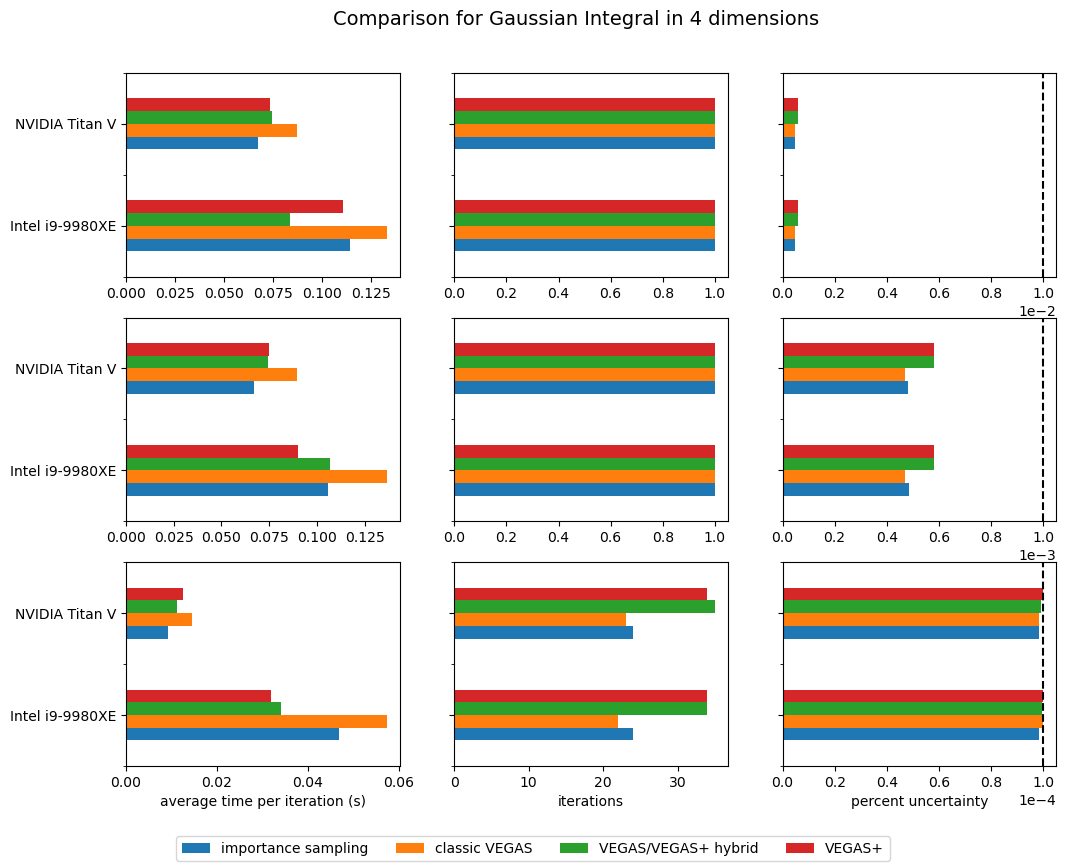
\includegraphics[width=\textwidth]{../images/gauss4d_final.png}
	\caption{Benchmark  for the integral $I_4$ in Eq.\eqref{gauss_example}. From right to left are presented the average time per iteration (after the warm-up), the number of iterations needed to reach target accuracy and the percent uncertainty reached at the end of the simulation. From the first row to the last one the target accuracies (dashed in the last column) are at $10^{-2}$, $10^{-3}$ and $10^{-4}$ percent uncertainty.}
	\label{gauss4d}
\end{figure}
In Fig.\ref{gauss4d} we can observe the benchmark results for dimension 4.
For a percent uncertainty of $10^{-2}$  or $10^{-3}$ all the algorithms converge in only 1 iteration after the warm-up. Looking at the accuracy reached the importance sampling and the classic VEGAS  are slightly more precise compared to the VEGAS+ algorithms.

In the last row of the plot we can see the results with a target accuracy of $10^{-4}$ percent uncertainty. 
This time all the algorithms converge within 40 iterations. The classic VEGAS integrator converges using a couple of  iterations less compared to the importance sampling of \texttt{VegasFlow}. The VEGAS+ integrators need more iterations to reach the target accuracy.

We can easily explain this behaviour since the integral in Eq.\eqref{gauss_example} is separable. Moreover, there is a sharp peak at the center of the integration region which favours the importance sampling. VEGAS+ is not effective in this case since we are not dealing with diagonal-structured integrands.

The average time per iteration (first column of the plot) is fairly similar for all the integrators even if the classic VEGAS algorithm, which converge in less iterations, seem to be the slower one. All the newly implemented integrators show better performances when running on GPU compared to the CPU. In particular, for the classic VEGAS integrator we observe a 3x improvements when running on the Titan V.
\subsection{Dimension 8}
\begin{figure}
	\centering
	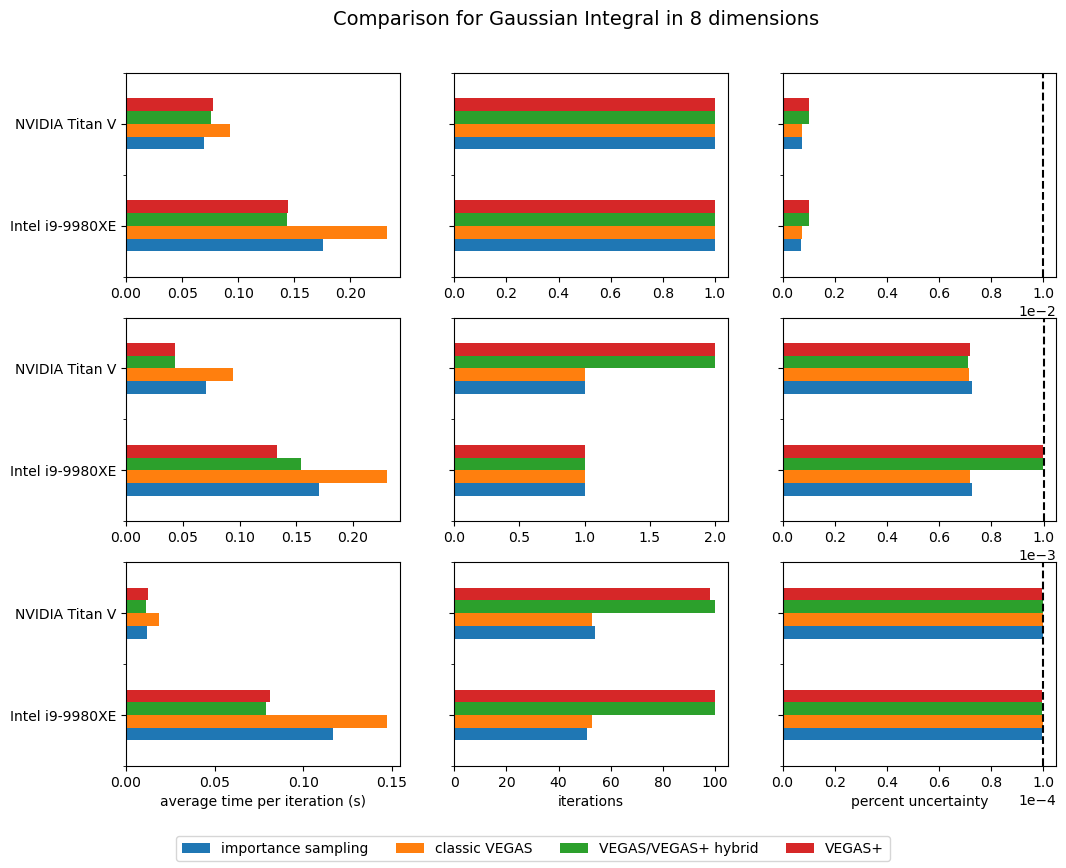
\includegraphics[width=\textwidth]{../images/gauss8d_final.png}
	\caption{Benchmark  for the integral $I_8$ in Eq.\eqref{gauss_example}. From right to left are presented the average time per iteration (after the warm-up), the number of iterations needed to reach target accuracy and the percent uncertainty reached at the end of the simulation. From the first row to the last one the target accuracies (dashed in the last column) are at $10^{-2}$, $10^{-3}$ and $10^{-4}$ percent uncertainty.}
	\label{gauss8d}
\end{figure}
In Fig.\ref{gauss8d} are presented the result for the integral $I_n$ of Eq.\eqref{gauss_example} with $n = 8$.

The trend is similar to the previous case studied. As expected the importance sampling and the classic VEGAS are the better performing 
integrators. In fact, they converge using less iterations particularly for a percent uncertainty of $10^{-4}$ where they converge using 50-60 iterations compared to the 98-100 iterations of  VEGAS+ and VEGAS/VEGAS+ hybrid.

By looking at the average time per iteration we can observe that the VEGAS+ algorithms, i.e. the VEGAS-VEGAS+ hybrid and VEGAS+,  are the fastest when running on CPU.  We expect similar results for the running time, in fact, excluding the warm-up phase all the new integrators converge in around 8 seconds. The \texttt{VegasFlow} integrator converges to the required accuracy in 5 seconds since the average time per iterations is better compared to
the classic VEGAS one.

In a GPU environment we can see great improvements especially when the simulation involves a larger number of iterations.
This is expected since, as discuss in Sect.\ref{tensorflow},  the graph-mode implementation of TensorFlow  is more effective when a function is called a large number of times. The importance sampling and the classic VEGAS integrators exhibit a 10x and a 8x improvement respectively in the average time per iterations, while the VEGAS+ algorithms show a speed-up by a factor 6.5.

 
 \subsection{Dimension 12}
 Next we move to dimension 12 by considering the integral $I_n$ of Eq.\eqref{gauss_example} with $n = 12$.
 
 For lower accuracies we can see that all the integrators converge using roughly the same number of iterations. For the case of a target accuracy of $10^{-4}$ relative tolerance the integrators exhibit different behaviours. The importance sampling and the classic VEGAS algorithms reach the accuracy required using the same number of iterations. We observe that more iterations are required on GPU but this is somewhat expected since we are dealing with MC integrators, therefore the number of iterations for the same algorithm can vary.
 
The VEGAS/VEGAS+ hybrid and the VEGAS+ integrators have more difficulty reaching the desired accuracy. This is due to the fact that 
stratified techniques become ineffective at higher dimensions. The adaptive stratified sampling aims at exploring the integration domain faster by redistributing the samples. For the case of a 12-dim Gaussian, due to the large integration domain, the redistribution can move away points from the peak resulting in a slower converge of the integral estimate. 
For the VEGAS/VEGAS+ hybrid, where the redistribution is stopped after the 5 warm-up iterations, it can happen that during the last redistribution the points are distributed in a less optimal configuration. This may explain the fact when running on CPU the VEGAS/VEGAS+ hybrid cannot reach the desired accuracy after the maximum number of iterations set to $1000$.

Looking at the average time per iteration the results show a pattern similar to the 8-dim Gaussian. The speed-up factors, for the higher precision case, are the following: importance sampling 11.5, classic VEGAS 10.1, VEGAS/VEGAS+ hybrid 14.8 and VEGAS+ 7.8.
The significant improvement in VEGAS/VEGAS+ is mainly due to the odd result observed when running on CPU, the other ones are similar to the previous cases.

\begin{figure}
	\centering
	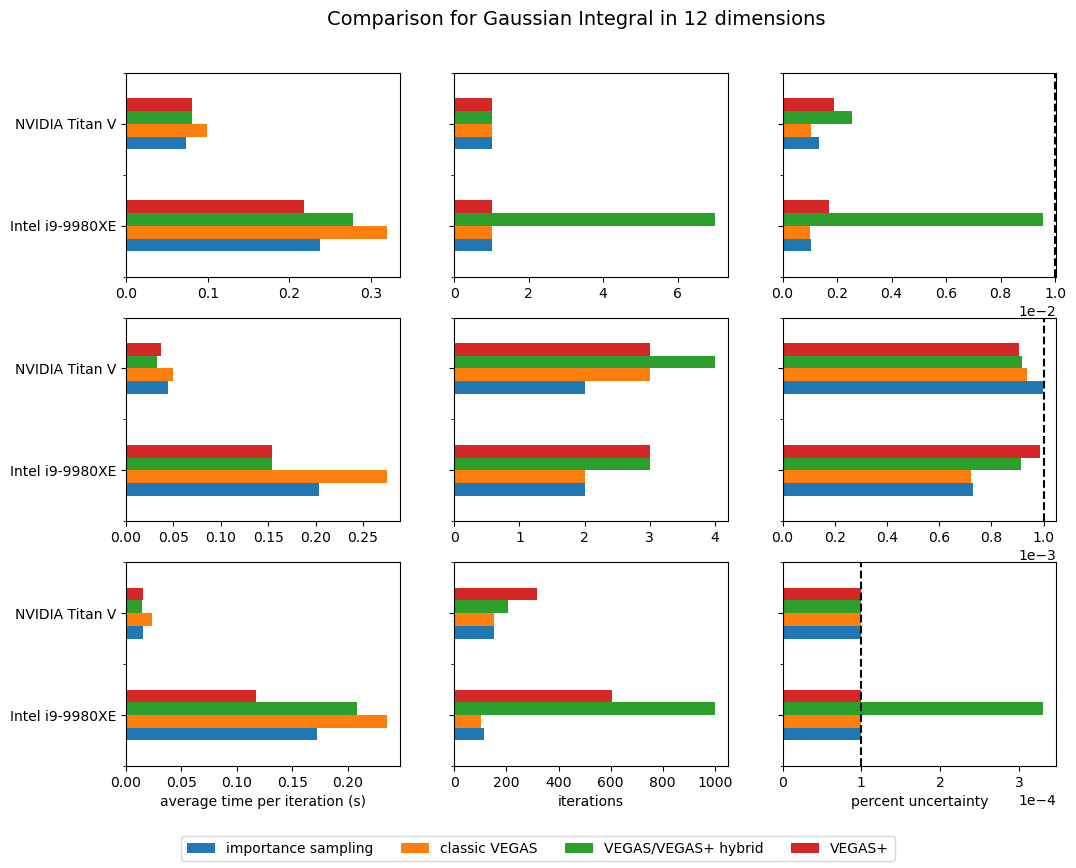
\includegraphics[width=\textwidth]{../images/gauss12d_final.png}
	\caption{Benchmark  for the integral $I_{12}$ in Eq.\eqref{gauss_example}. From right to left are presented the average time per iteration (after the warm-up), the number of iterations needed to reach target accuracy and the percent uncertainty reached at the end of the simulation. From the first row to the last one the target accuracies (dashed in the last column) are at $10^{-2}$, $10^{-3}$ and $10^{-4}$ percent uncertainty.}
	\label{gauss12d}
\end{figure}


\section{HEP integrands}
We also benchmark the performance of the new algorithms on integrands taken from particle physics processes.
The motivation behind this choice is that we are concerned by the computation cost of fixed order calculation involved in the simulation
of important experiments such as ATLAS or CMS, as already discussed in Section \ref{cost}.

We are interested in seeing if any of the new implemented integrators can perform better than the importance sampling of \texttt{VegasFlow} in the computation of physical integrals.

In particular according to modern amplitude methods we use the spinor helicity formalism described in Ref\cite{Dixon:1613349}. We no longer consider the four-momenta of the particles $k_i^\mu$, since the majority of the particle in the Standard Model have spin, but we work with a smaller representation of the Lorentz group, the spinor representation.
    
\subsection{Drell-Yan process}

\begin{figure}
	\centering
	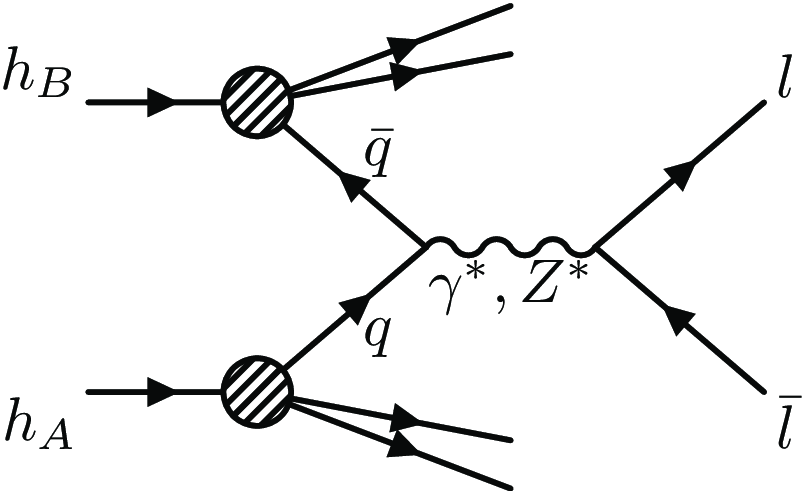
\includegraphics[width=6cm]{../images/Drell-Yan-process-a-quark-of-one-hadron-and-an-antiquark-of-another-hadron-annihilate.png}
	\caption{Representation of the DY process at LO. Image from Ref\cite{article}.}
	\label{DY}
\end{figure}
The first example that we consider is the Drell-Yan (DY) process, which consists in an inclusive production of high-mass lepton pairs in hadron-hadron collision:
\begin{equation}
	h_A + h_B \rightarrow ( \gamma^* + l \bar{l}) + X 
\end{equation}
where $X$ is an undetected final state, as shown in Fig.\ref{DY}.

In particular we consider the aforementioned process at the partonic level, this is, without considering the convolution with the parton density functions. We use the expression for the cross section computed at LO take from Ref\cite{Carrazza_2020}.

The benchmark results are shown in Fig.\ref{pineappl_plot}. 

As for the previous cases, at lower accuracies all the integrators converges using less the 3 iterations. We can observe that the importance sampling and the classic VEGAS at a percent uncertainty of 0.001\% reach the target accuracy using only one iteration after the warm-up.
This trend continues for higher accuracies where there is a major different in the number of iterations needed to satisfy the precision requirements. Classic VEGAS is the better performing integrator compared to the importance sampling. The VEGAS+ algorithms have a more difficult time reaching the desired accuracy, they can need up to 5 times the number of iterations required to the classic VEGAS integrator.

Regarding the average time per iteration, the importance sampling is the fastest integrators followed by the classic VEGAS algorithm. The other integrators can take up to twice the time when running on GPU compared to the faster ones. All the integrators show a better performance when running on GPU compared to CPU. The importance sampling and the classic VEGAS methods have a speed-up factors of 7.7 and 6 respectively.

The worst performance of the VEGAS+ methods suggests that the integral doesn't have multiple peaks, but rather a sharp peak which is easily found by the VEGAS grid. 


\begin{figure}[]
	\centering
	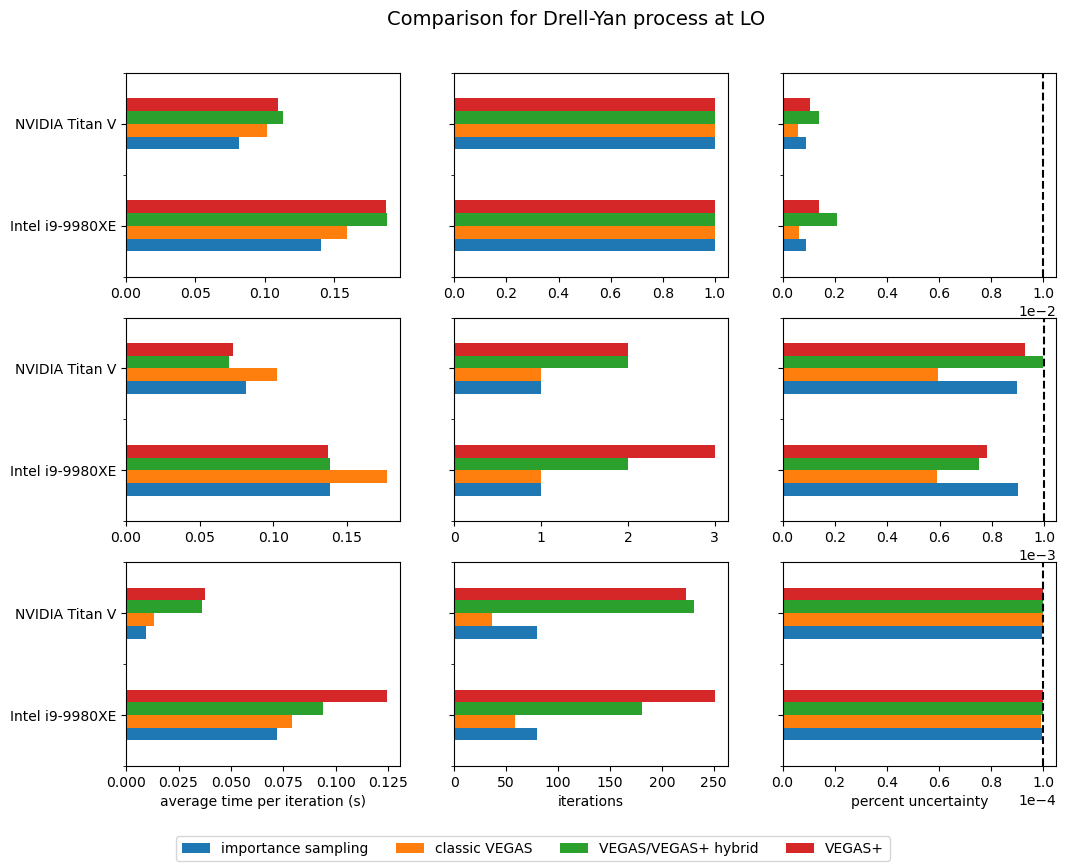
\includegraphics[width=\textwidth]{../images/pineappl_final.png}
	\caption{Benchmark  for the partonic level cross section for the DY photon induced process  at LO \cite{Carrazza_2020}. From right to left are presented the average time per iteration (after the warm-up), the number of iterations needed to reach target accuracy and the percent uncertainty reached at the end of the simulation. From the first row to the last one the target accuracies (dashed in the last column) are at $10^{-2}$, $10^{-3}$ and $10^{-4}$ percent uncertainty.}
	\label{pineappl_plot}
\end{figure}





\subsection{Single Top Production}
\label{singletop_sect}
Another interesting process to consider is the production of the $t$-quark since it is important for understanding many properties such as the top quark mass, his  Cabbibo-Kobayashi-Maskawa matrix element $V_{tb}$ and many others.

Although the top quark is mainly produced via to the strong interactions, we consider his production governed by the weak interactions since it is relevant for several events at the LHC. There are several experimentally distinguishable ways to produce the single top quark, in this thesis we consider the $t$-channel process 
\begin{equation}
	\label{singletop}
	W^* b \to t 
\end{equation}
which has the largest cross section with  $\sqrt{s} = 8$ TeV at the LHC \cite{Brucherseifer_2014}.

In particular we consider the process of Eq.\eqref{singletop} at LO at the partonic level. The physical parameters chosen are $m_t = 173.2$ GeV and $\sqrt{s} = 8$ TeV.

The results are shown in Fig.\ref{singletop_plot}.
Even though this integral has the same dimension of the previous one we can see that the plots exhibit significant differences.
In the first place, for lower accuracies even if all the integrators converge in only 1 iterations after the warm-up VEGAS+ seem to be the faster both on GPU and CPU. 

This happens also at a higher accuracy on CPU, while on GPU the importance sampling of \texttt{VegasFlow} is the fastest methods looking at the average time per iterations. In fact, the importance sampling has a speed-up factor of 10.9 compared to the 4.32 of VEGAS+.

The most interesting aspect for this integral is the number of iterations needed to reach an accuracy of 0.0001\% percent uncertainty.  This is the first case where we see that the importance sampling alone is by far the less efficient method. Both on GPU and CPU \texttt{VegasFlow} needs at least 50 iterations to reach the required precision. On the other hand, all the new implemented algorithms converge using less than 10 iterations and VEGAS+ is the most accurate overall.

We can conclude that the adaptive stratified sampling technique of VEGAS+ seem to be particularly suited for the single-top production integrand.

\begin{figure}[]
	\centering
	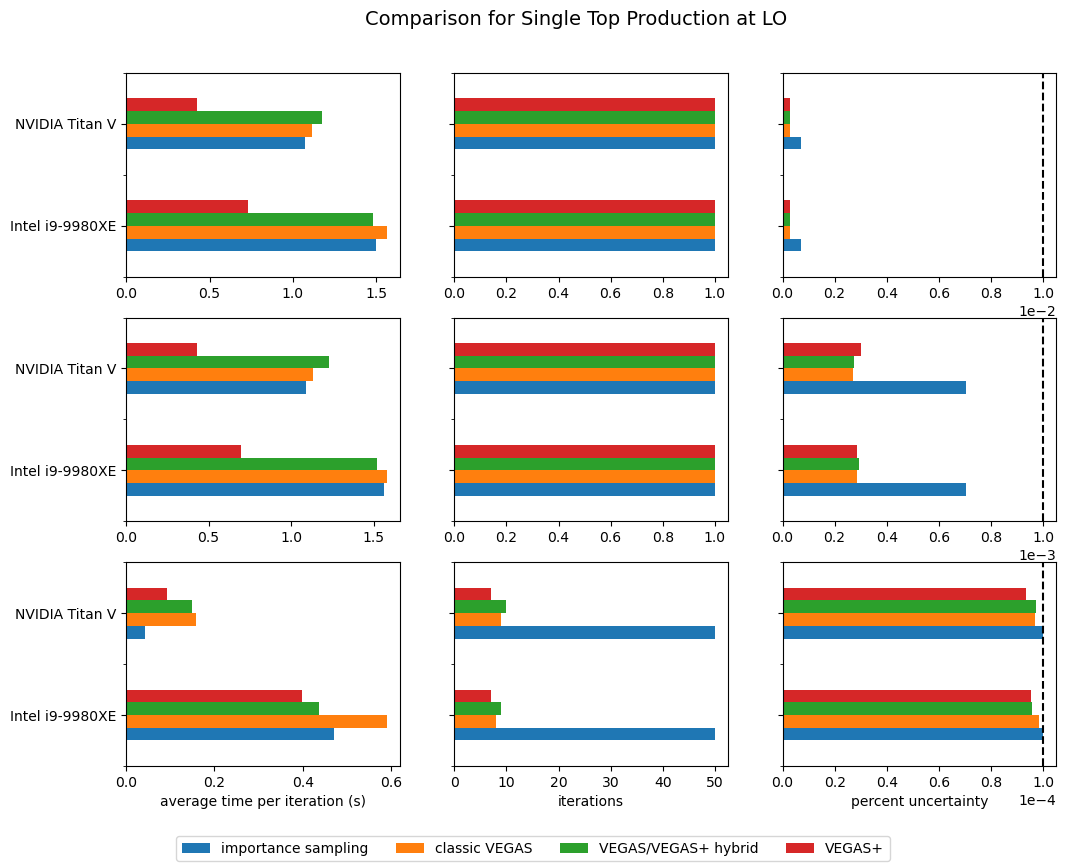
\includegraphics[width=\textwidth]{../images/singletop_final.png}
	\caption{Benchmark  for the partonic level cross section for the single $t$-quark production (t-channel)  at LO \cite{Brucherseifer_2014}. From right to left are presented the average time per iteration (after the warm-up), the number of iterations needed to reach target accuracy and the percent uncertainty reached at the end of the simulation. From the first row to the last one the target accuracies (dashed in the last column) are at $10^{-2}$, $10^{-3}$ and $10^{-4}$ percent uncertainty.}
	\label{singletop_plot}
\end{figure}
 
\subsection{Vector Fusion Boson Production Higgs at LO}

\begin{figure}[]
	\centering
	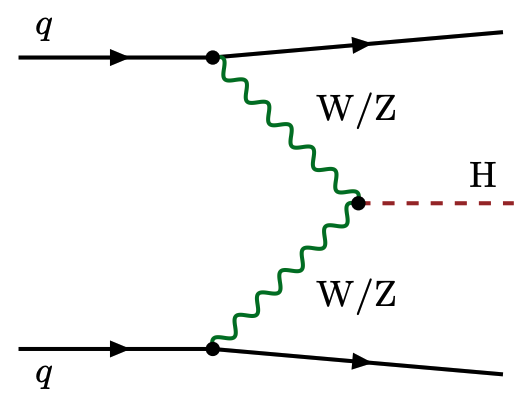
\includegraphics[width=5cm]{../images/vfb_image.png}
	\caption{ Born-level vector boson fusion process. Image from Ref\cite{Cruz_Martinez_2018}.}
	\label{vfb}
\end{figure}

Next we study a more complicated involving the Higgs boson $H$, which can be produced at the LHC through its Yukawa coupling to the top quark or through its coupling to electroweak bosons. In particular we consider the vector fusion boson process shown in Fig.\ref{vfb} which is the second-largest inclusive production mode for Higgs bosons, amounting to about 10\% of the dominant gluon fusion process \cite{Cruz_Martinez_2018}.

For this process we don't just compute the integral at the partonic level, but we also include the convolution with the PDFs. 
The parton density functions are including in the \texttt{VegasFlow} environment using the \texttt{PDFFlow} software \cite{Carrazza_2021,juan_m_cruz_martinez_2021_4903010}, which is implemented using the TensorFlow library and enable us to evaluate a generic set of PDFs on GPU. 
The integrand used is taken from Ref\cite{juan_m_cruz_martinez_2021_4903010}.

The results are shown in Fig.\ref{higgs_plot}.

Looking at the number of iterations needed to reach the target accuracy we can observe that the classic VEGAS algorithm is the more efficient integrator both at low and high precisions. The importance sampling method cannot outperform the other integration algorithms and in some cases struggle to converge to the required accuracy. This is interesting since we are computing a multi-dimensional integral of dimension 6. Usually we expect that the (adaptive) stratified sampling techniques have only small effects for high-dimensional integrals.

For the computational times we can observe how the average time per iterations decreases both on GPU and CPU if we consider more iterations, i.e. by going for higher precisions. The first iteration can take up to 6 seconds and we can reduce the average time per iterations to a few tenths of a second thanks to hardware acceleration and to the graph mode implementation of TensorFlow.

Regarding the average time per iteration, we can see that VEGAS+ and VEGAS/VEGAS+ hybrid are the fastest integrators, followed by the importance sampling and the classic VEGAS algorithm. We also observed significant improvements when the integration run on GPU with speed-up factors between 6 and 4.

 






\begin{figure}[h]
	\centering
	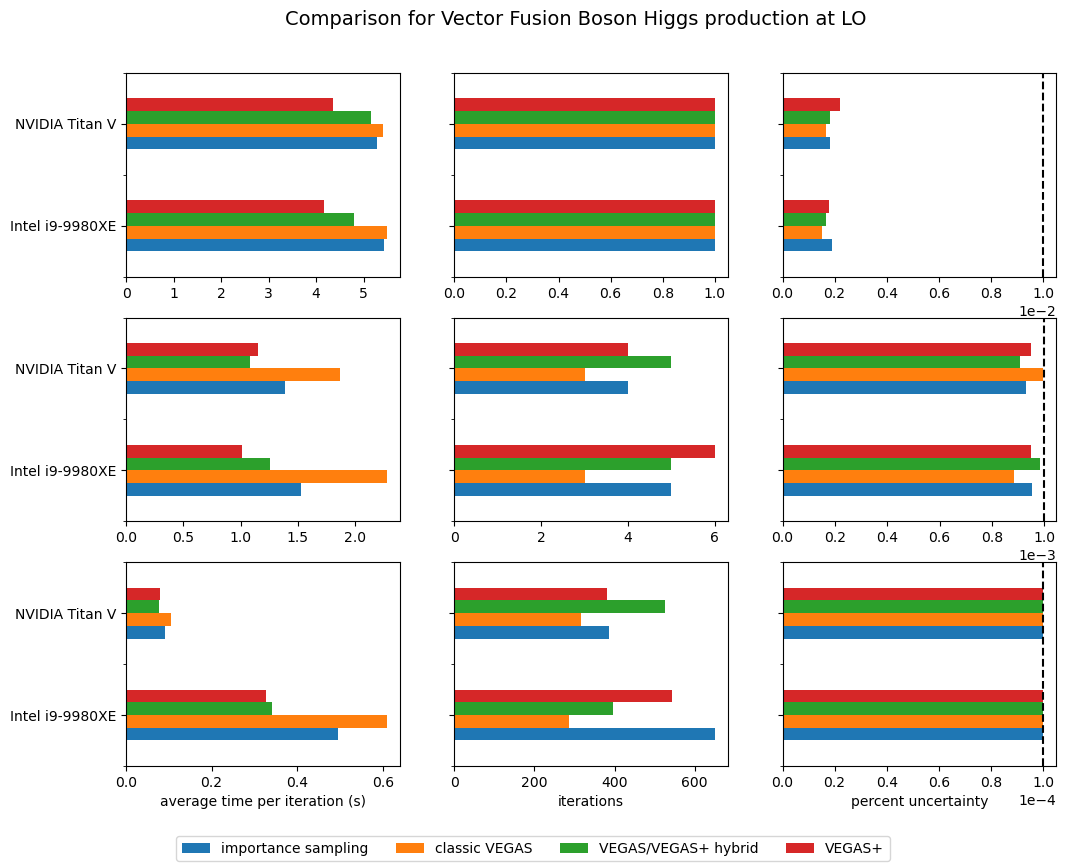
\includegraphics[width=\textwidth]{../images/higgs_LO_final.png}
	\caption{Benchmark  for the cross section for the vector fusion boson (VFB) Higgs production at LO \cite{Brucherseifer_2014}. The set of PDFs is \texttt{NNPDF31\_nnlo\_as\_0118/0} From right to left are presented the average time per iteration (after the warm-up), the number of iterations needed to reach target accuracy and the percent uncertainty reached at the end of the simulation. From the first row to the last one the target accuracies (dashed in the last column) are at $10^{-2}$, $10^{-3}$ and $10^{-4}$ percent uncertainty.}
	\label{higgs_plot}
\end{figure}

\section{Recipe for the reader}
We now compare all the results obtained in the previous section. We would like to see if we can suggest to the user which integrators works best depending on the integral to compute. We base this analysis on the average time per iteration and on the number of iterations needed for the precision of 0.0001\% percent uncertainty.

\subsection{Average time per iteration}
In Fig.\ref{cpu_time_comparison} we show the average time per iteration (after the warm-up) for all the integrands used in the benchmark when running on the Intel i9-9980XE.

As expected all the integrators requires more time per iteration when computing the single top and the higgs production due to the more complex integrands to evaluate. However, it is interesting to observe that for the previous cases the average time per iteration is shorter for the two VEGAS+ algorithms compared to the classic VEGAS and the importance sampling of \texttt{VegasFlow}.
This is very important for our analysis since we are concerned by the CPU usage when integrating physical integrands. 

The same cannot be said for the DY integral although we can observe that the time differences in all the integrators is quite limited due to the low-dimensional integration domain.

By looking at the standard gaussian integrals for all the integrators the time increases as the dimension increases which is expected. Furthermore, the plot shows that using the VEGAS+ integrator the average time per iteration is almost always shorter compared to all the other integrators. This is true even for the 12-dim gauss integral despite the high dimension.


\begin{figure}[h]
	\centering
	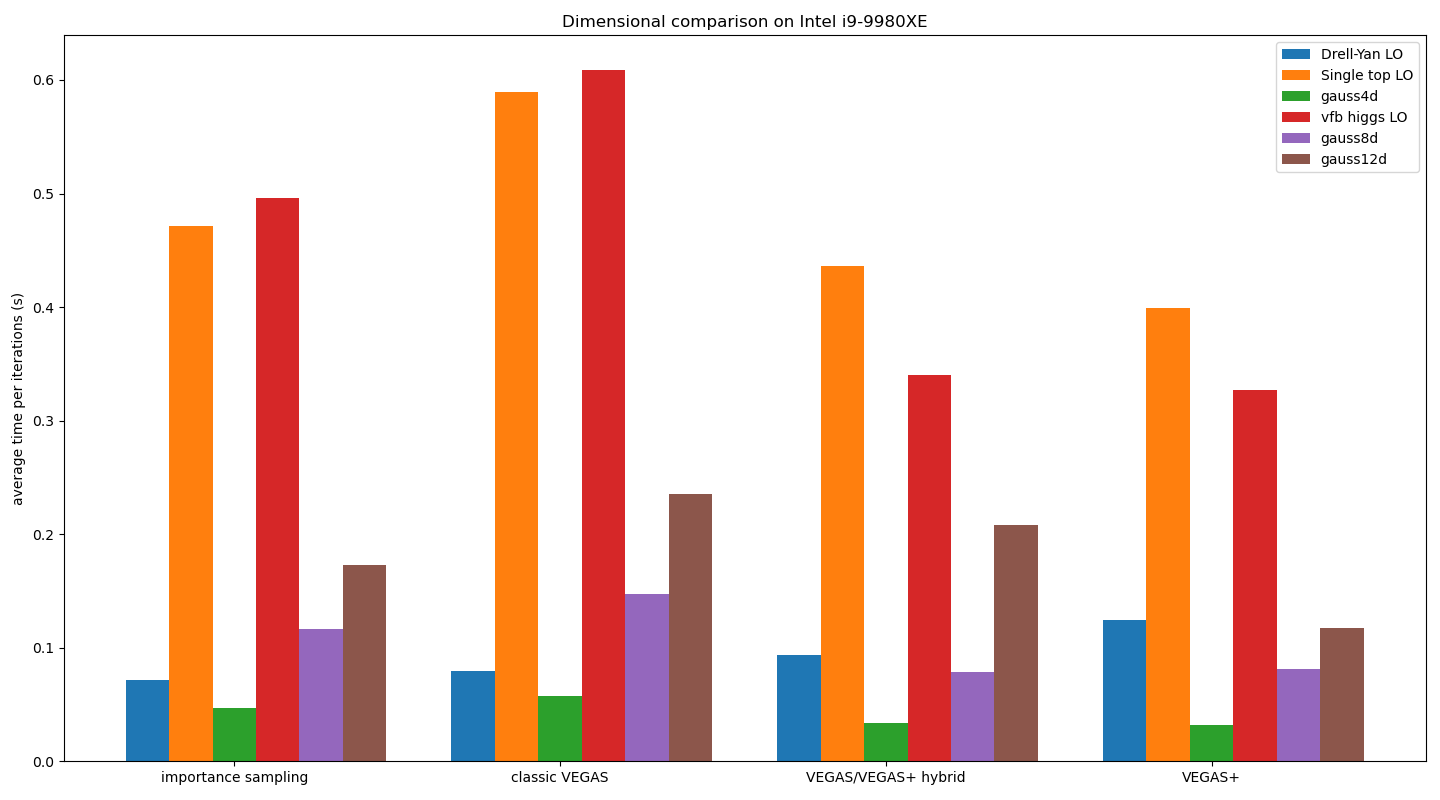
\includegraphics[width=\textwidth]{../images/dim_comparison_CPU.png}
	\caption{Average time per iterations (after the warm-up) for all the previously studied cases. The results are sorted by the integrand dimension for each integrator. All the integration are performed on the Intel i9-9980XE CPU. }
	\label{cpu_time_comparison}
\end{figure}

In Fig.\ref{gpu_time_comparison} we present the same plot when all the integrations are performed on the NVIDIA Titan V GPU. We can see that all the times are shortened and have similar values except for the more complicated integrals (single top and higgs production).

Overall the fastest integrator seem to be the importance sampling. In fact, there is a great improvement on the computational time of the single top integral compared to the CPU case. That same time cannot be reached by the other integrators when running on GPU.

The case of the VFB Higgs production is also interesting. The VEGAS/VEGAS+ hybrid and the VEGAS+ algorithms are faster than the importance sampling as for the CPU case. This means that the new integrators can provide a solid alternative in a GPU environment when computing complicated physical integrands.

\begin{figure}[h]
	\centering
	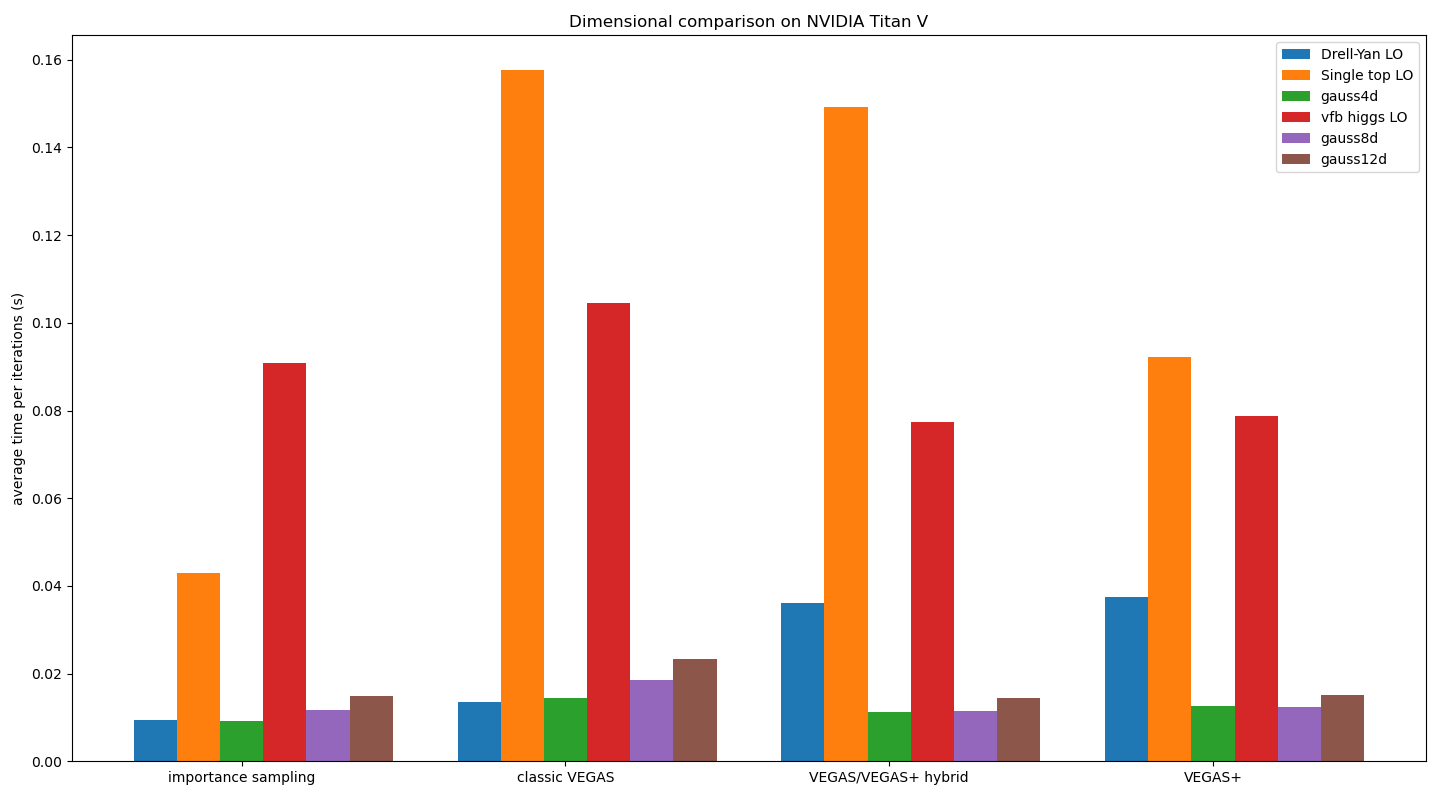
\includegraphics[width=\textwidth]{../images/dim_comparison_GPU.png}
	\caption{Average time per iterations (after the warm-up) for all the previously studied cases. The results are sorted by the integrand dimension for each integrator. All the integration are performed on the NVIDIA Titan V GPU. }
	\label{gpu_time_comparison}
\end{figure}


\subsection{Number of iterations}
We consider now the number of iterations needed to reach the target accuracy of 0.0001 percent uncertainty for all the previous integrands. Since the number of iterations are independent on the hardware environment (CPU or GPU) we have decided to present the results from the integration on CPU. 

The results are shown in Fig.\ref{cpu_iter_comparison}. The integrator that in general converge
using less iterations is the classic VEGAS algorithm, i.e. without the redistribution of samples. It is more accurate than the importance sampling for all the physical integrands: DY, single top and Higgs production. In fact, for the Higgs production integrand classic VEGAS converges using less than half iterations used by the importance sampling.

For the single top production all the new implemented algorithms can outperform the importance sampling, as already observed in Section \ref{singletop_sect}.

As expected the adaptive stratified sampling methods needs more iterations as the dimensionality of the integrands increases, especially if the peaks are easy to find by the VEGAS grid, as for the case of a Gaussian distribution with a single peak.
\begin{figure}[h]
	\centering
	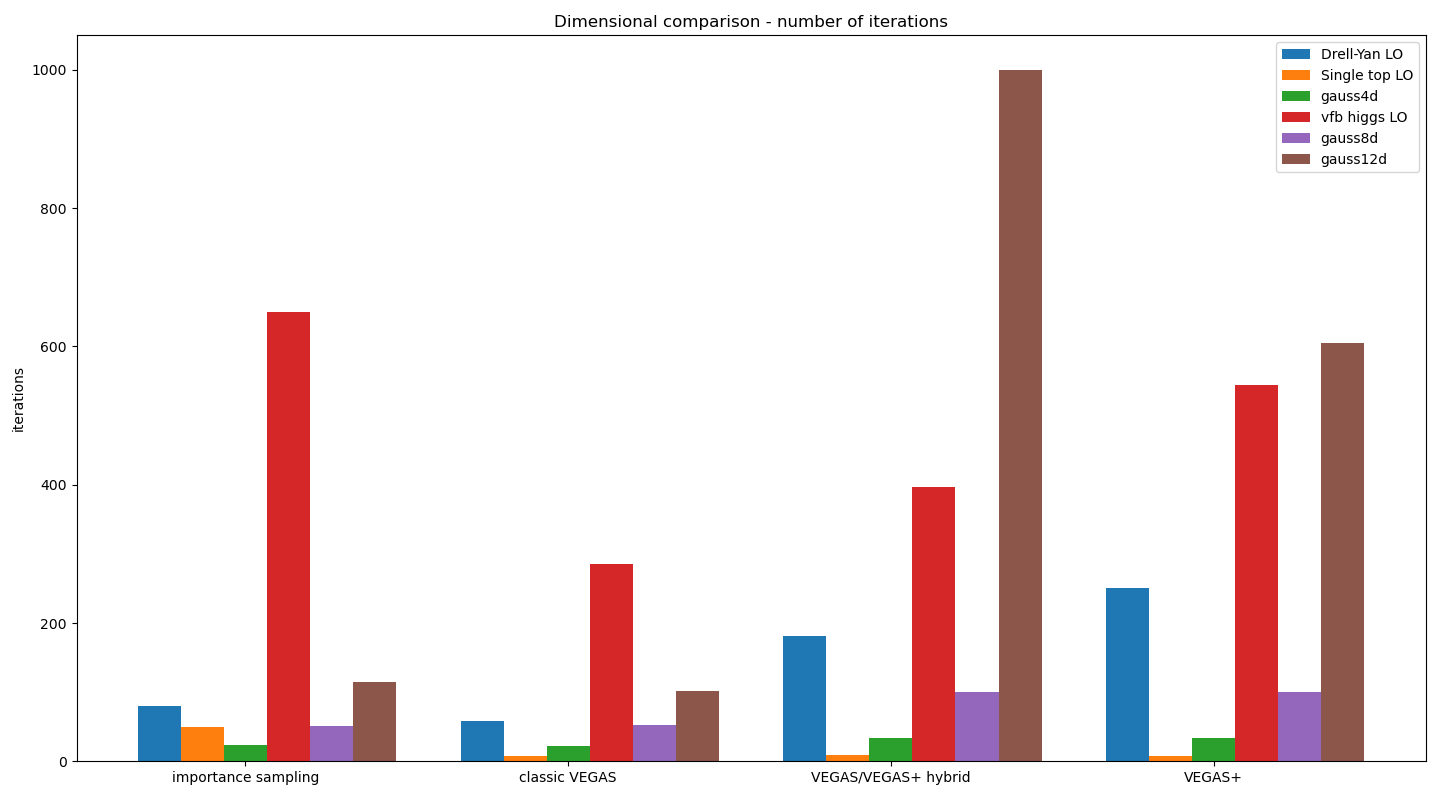
\includegraphics[width=\textwidth]{../images/dim_comparison_iter.png}
	\caption{Iterations needed to reach the accuracy of $10^{-4}$ percent uncertainty (after the warm-up) for all the previously studied cases. The results are sorted by the integrand dimension for each integrator. All the integration are performed on the Intel i9-9980XE CPU. }
	\label{cpu_iter_comparison}
\end{figure}

\subsection{Final comments}
The newly implemented integrators in the \texttt{VegasFlow} library provide solid alternatives to the importance sampling algorithm already implemented in the library.

By looking at the average time per iterations,we have shown that the integrators that employs the VEGAS+ algorithms can outperform the importance sampling method when dealing with high-dimensional and complicated integrals such as the VFB Higgs production.
For the case of gaussian integration all the integrators exhibit the same performance, especially on GPU, with a few differences on CPU that seem to favour the VEGAS+ algorithms.

For low-dimensional physical integrands such as the DY and the single top production the importance sampling perform better especially in the case of the DY process both on CPU and GPU.
In computing the single top integral the importance sampling  performs better on GPU while on CPU the VEGAS+ algorithm seem to be the fastest.

When comparing the number of iterations we have observed that the classic VEGAS is the more efficient integrator in general. Therefore, even if his computational time are not as fast the other integrators, is still a valuable option since the simulation will require less iterations. 

The VEGAS/VEGAS+ hybrid and the VEGAS+ algorithms converge using a small number of iterations when integrating physical integrands such as the single top or the Higgs production. This, combined with the short average times per iteration on CPU and on GPU, makes these methods a very useful tool when computing particle process related integrals.



	
\end{document}